\section{内存管理}

内存管理机制是实时操作系统的重要组成部分。操作系统通过页表机制实现了对内存空间的控制。页表使得 xv6 能够让不同进程各自的地址空间映射到相同的物理内存上,还能够为不同进程的内存提供保护。除此之外,我们还能够通过使用页表来间接地实现一些特殊功能。xv6 主要利用页表来区分多个地址空间,保护内存。另外,它也使用了一些简单的技巧, 即把不同地址空间的多段内存映射到同一段物理内存(内核部分),在同一地址空间中多次映射同一段物理内存(用户部分的每一页都会映射到内核部分),以及通过一个没有映射的页保护用户栈。下面我们就来详细介绍一下 xv6 的内存管理.

xv6 初始化之后的物理内存图:

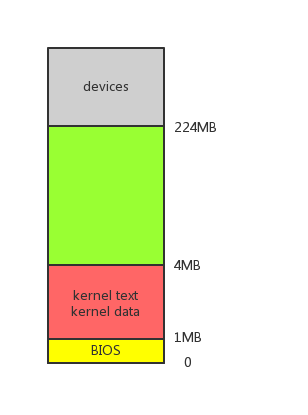
\includegraphics[width=6in]{figures/mem/fig1.png}

下面这个图展示的是 XV6 中虚拟地址到物理地址的映射关系.

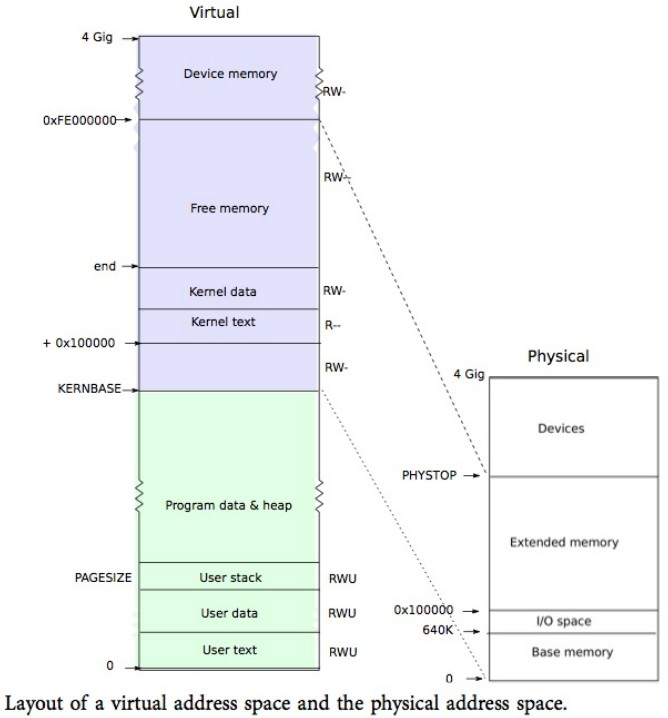
\includegraphics[width=6in]{figures/mem/fig2.png}

xv6 使用页表(由硬件实现)来为每个进程提供其独有的地址空间。页表将虚拟地址(x86 指令所使用的地址)翻译(或说“映射”)为物理地址(处理器芯片向主存发送的地址).  Xv6实现了两级页表, 第一级页表有 1024 项 (占有 4096 字节), 第二级页表也有 1024 项 (占有4096 字节), xv6 为每一个进程分配了这样的一个二级页表来实现将进程的虚拟地址转化为物理地址的过程. 分页硬件使用虚拟地址的高 10 位来决定对应页目录条目。如果想要的条目已经放在了页目录中,分页硬件就会继续使用接下来的 10 位来从页表页中选择出对应的 PTE。否则,分页硬件就会抛出错误。通常情况下,大部分虚拟地址不会进行映射,而这样的二级结构就使得页目录可以忽略那些没有任何映射的页表页。在分页机制之中, 虚拟地址的高 20 位来找到该虚拟地址在页表中的索引,然后把其高 20 位替换为对应 PTE 的 PPN。而低 12 位

是会被分页硬件原样复制的。因此在虚拟地址-物理地址的翻译机制下,页表可以为操作系统     提供对一块块大小为 4096(2ˆ12)字节的内存片,这样的一个内存片就是一页。

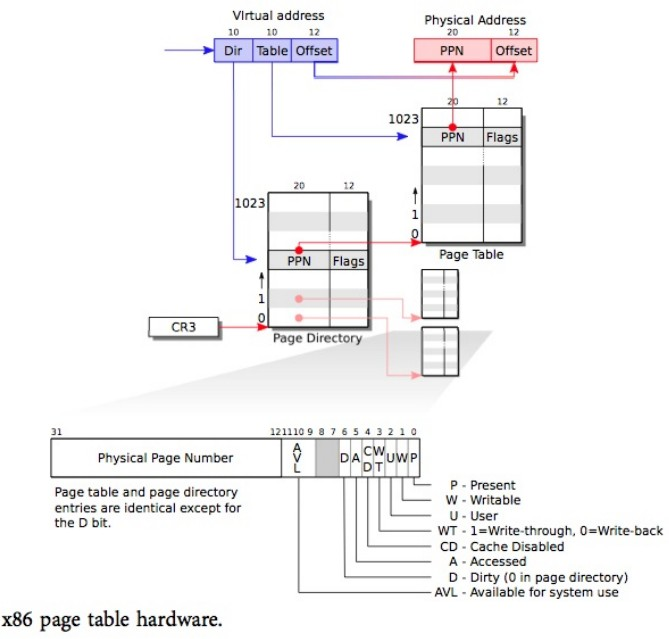
\includegraphics[width=6in]{figures/mem/fig3.png}

从图中可以看到, 每个 PTE 都包含一些标志位,说明分页硬件对应的虚拟地址的使用权限。PTE\_P 表示 PTE 是否陈列在页表中:如果不是,那么一个对该页的引用会引发错误(也就是:不允许被使用)。PTE\_W 控制着能否对页执行写操作;如果不能,则只允许对其进行读操作和取指令。PTE\_U 控制着用户程序能否使用该页;如果不能,则只有内核能够使用该页。图 2-1 对此进行了说明。这些的标志位和页表硬件相关的结构体都在 mmu.h 定义。

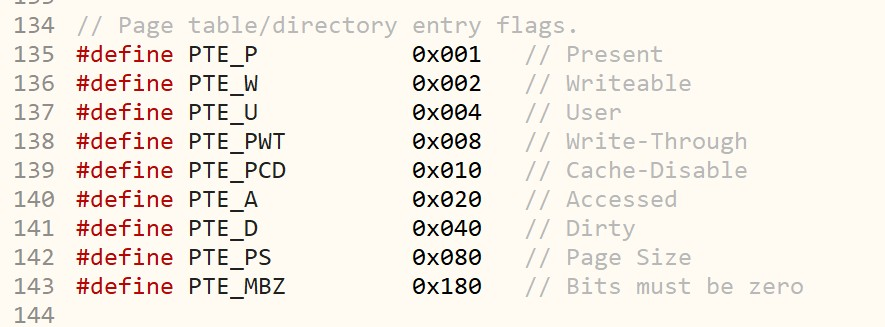
\includegraphics[width=6in]{figures/mem/fig4.png}

每个进程都有自己的页表,xv6 会在进程切换时通知分页硬件切换页表。如图所示,

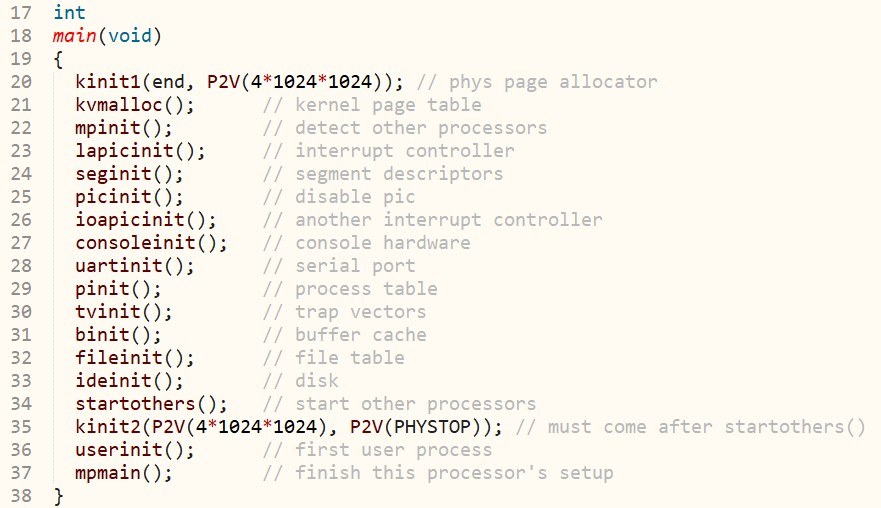
\includegraphics[width=6in]{figures/mem/fig5.png}

进程的用户内存从 0 开始,最多能够增长到 KERNBASE , 这使得一个进程最多只能使用 2GB 的内存。当进程向 xv6 要求更多的内存时,xv6 首先要找到空闲的物理页,然后把这些页对应的  PTE  加入该进程的页表中,并让  PTE  指向对应的物理页。xv6  设置了PTE 中的 PTE\_U、PTE\_W 、PTE\_P 标志位。大多数进程是用不完整个内存空间的;xv6 会把没有被使用的 PTE 的 PTE\_P 标志位设为 0。不同进程的页表将其用户内存映射到不同的物理内存中,因此每个进程就拥有了私有的用户内存。xv6 在每个进程的页表中都包含了内核运行所需要的所有映射,而这些映射都出现在  KERNBASE  之上。它将虚拟地址KERNBASE:KERNBASE+PHYSTOP  映射到   0:PHYSTOP  。这样映射的原因之一是内核可

以使用自己的指令和数据;原因之二是内核有时需要对物理页进行写操作,譬如在创建页表页的时候,而使得每一个物理页都在对应的虚拟地址上被映射就让这些操作变得很方便。这样的安排有一个缺点,即 xv6 无法使用超过 2GB 的物理内存。有一些使用内存映射的 I/O 设备的物理内存在 0xFE000000 之上,对于这些设备 xv6 页表采用了直接映射。KERNBASE 之上的页对应的 PTE 中,PTE\_U 位均被置 0,因而只有内核能够使用这些页。每个进程的页表同时包括用户内存和内核内存的映射,这样当用户通过中断或者系统调用转入内核时就不需要进行页表的转换了。大多数情况下,内核都没有自己的页表,所以内核几乎都是在借用用户进程的页表。Xv6 如何建立一个地址空间代码分析在第 21 行 main 调用 kvmalloc 来创建并切换到一个拥有内核运行所需的 KERNBASE 以上映射的页表。

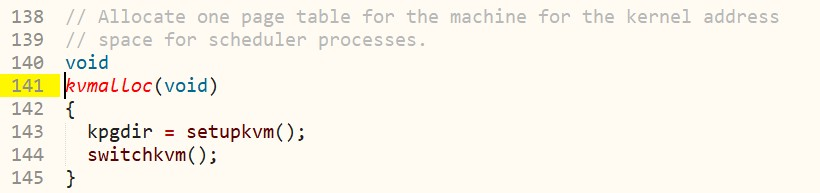
\includegraphics[width=6in]{figures/mem/fig6.png}

这里的大多数工作都是由 setupkvm 完成的。

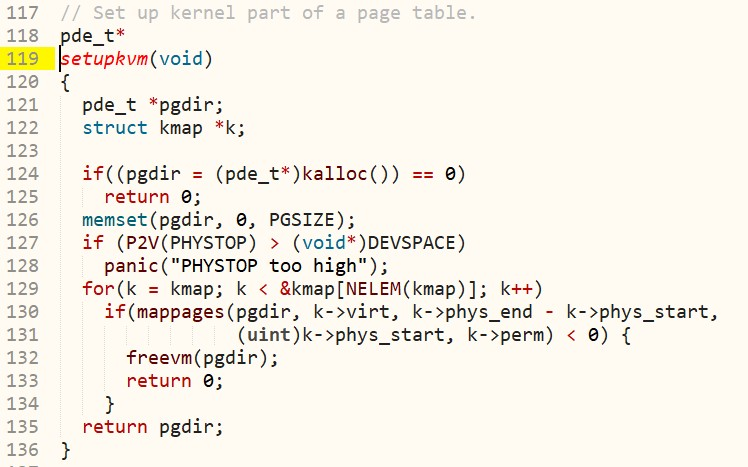
\includegraphics[width=6in]{figures/mem/fig7.png}

首先,它会分配一页内存来放置页目录,然后在第 130 行调用 mappages 来建立内核需要的映射,这些映射可以在 kmap 数组中找到。这里的映射包括内核的指令和数据,PHYSTOP 以下的物理内存,以及 I/O 设备所占的内存。setupkvm 不会建立任何用户内存的映射,这些映射稍后会建立。

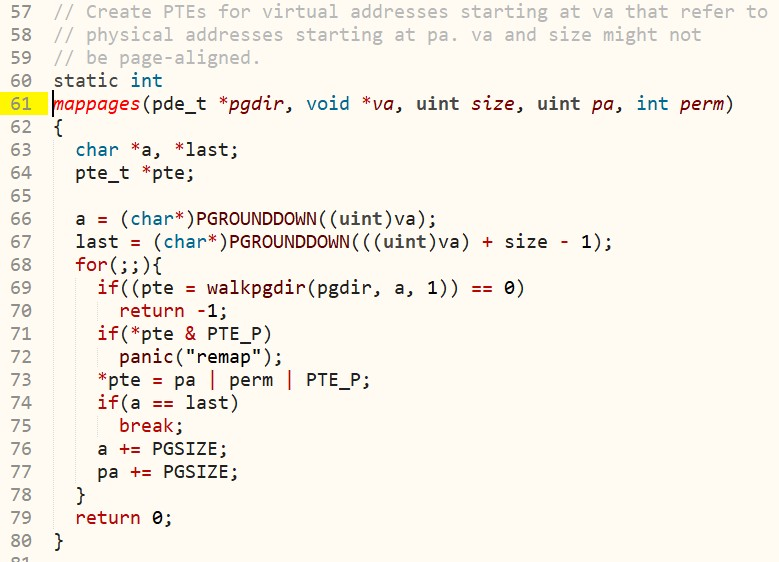
\includegraphics[width=6in]{figures/mem/fig8.png}

mappages 做的工作是在页表中建立一段虚拟内存到一段物理内存的映射。它是在页的级别,即一页一页地建立映射的。对于每一个待映射虚拟地址,mappages 调用 walkpgdir 来找到该地址对应的 PTE 地址。然后初始化该 PTE 以保存对应物理页号、许可级别(PTE\_W 和/或 PTE\_U )以及 PTE\_P 位来标记该 PTE 是否有效.

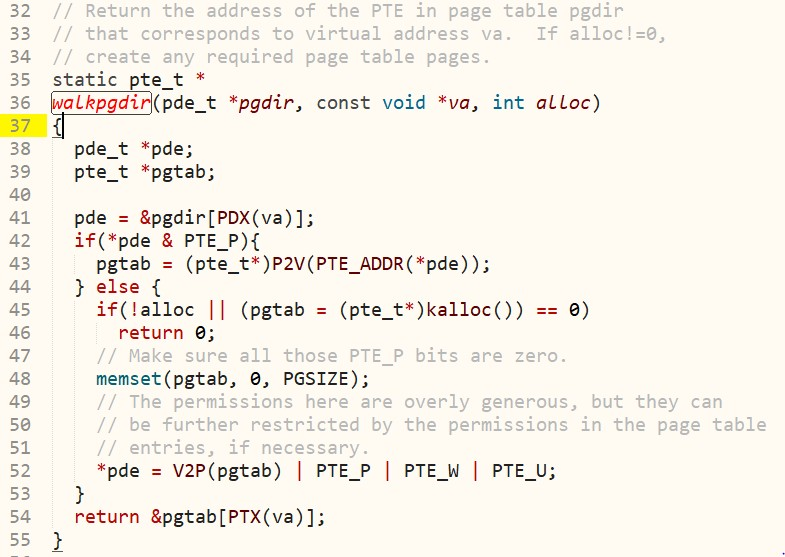
\includegraphics[width=6in]{figures/mem/fig9.png}

walkpgdir 模仿 x86 的分页硬件为一个虚拟地址寻找 PTE 的过程。walkpgdir 通过虚拟地址的前 10 位来找到在页目录中的对应条目,如果该条目不存在,说明要找的页表页尚未分配;如果 alloc 参数被设置了,walkpgdir 会分配页表页并将其物理地址放到页目录中。最后用虚拟地址的接下来 10 位来找到其在页表中的 PTE 地址. 物理内存的分配 Xv6 在运行时, 内核需要为页表、进程的用户内存、内核栈及管道缓冲区分配空闲的物理内存。xv6 使用从内核结尾到 PHYSTOP 之间的物理内存为运行时分配提供内存资源。每次分配,它会将整块
4096 字节大小的一页分配出去。xv6 还会通过维护一个物理页组成的链表来寻找空闲页。所以,分配内存需要将页移出该链表,而释放内存需要将页加入该链表。
